This section presents simulation results that show how the control inputs
obtained running the optimization of Section \ref{sec:motionP}, are able to bring the robot to a desired target. 
We used the OCP solver PINS~\cite{pins:1,pins:2,pins:3}, which relies on the indirect approach based on the Pontryagin Maximum Principle.
The code to replicate the results is freely available at \footnote{ \href{https://github.com/mfocchi/climbing\_robots.git}{https://github.com/mfocchi/climbing\_robots.git}}.

% 1st experiment: validation of optimization with 2 models, with obstacle
In a first experiment, we run the optimization to perform  a 12 $m$ long jump starting from an initial 
position $\vect{p}_0 = \mat{0.24& 0& -8}^T$ up to a target at $\vect{p}_f = \mat{3 & 3 &-20}^T$ $[m]$. As additional constraint,
during the jump, the robot has to avoid a rock pillar laying on the wall, that we model as a 20 $m$ high cone with a base of radius 2.5 $m$.
We validate the result of the optimization for both the simplified model (in a Matlab environment)
and the full 3D model. For this case we built a Gazebo simulator based on the URDF description \cite{urdf} of the robot (see Fig. \ref{fig:3dmodel}(right)).
Table \ref{tab:params} reports the used physical parameters, together with some optimization settings.
%
\begin{table}[!tbp]
	\centering
	\caption{ Simulations parameters}
		\begin{tabular}{l c c  } \hline\hline
			\textbf{Name} \quad                  & \textbf{Symbol}                     & \textbf{Value}  \\ \hline
					Robot mass                   & m  & 5                 \\ 
					Max. impulse  [N]       	 & $F_{u}^{\text{max}}$				& 1000   \\
					Max. retraction force [N]    & $F_r^{\text{max}} $			& 200    \\
					Friction coeff.				 & $ \mu $ 					        & 0.7   \\
					Thrust impulse duration	[s]  & 	$T_{th}$  				& 0.025\\
					Discretization steps         & N 						& 500\\					        
			\hline\hline 					    					    					    
		\end{tabular}
		\label{tab:params}
\end{table}
%
For the Matlab simulation we simply integrate~\eqref{eq:nonlinearDyn} 
with an ode45 Runge-Kutta variable-step scheme.
For the Gazebo simulation, we assume to apply the push impulse as a force $F_c$ at the contact point.
Therefore we employ the leg dynamics to define the mapping between the contact force $F_c$ and the torques $\tau_{\text{leg}}$ at the leg joints:
%
\begin{equation}
\boldsymbol{\tau}_{\text{leg}}^d= \mat{\tau_{HP} \\ \tau_{HR} \\ \tau_{K}} =  \vect{h}_{\text{leg}} -\vect{J}_{\text{leg}}^T \underbrace{\left(R_e^\mathcal{W}  \mat{F_{u,n} \\ F_{u,t} \\ 0} \right) 	}_{\vect{F}_c}
\end{equation}
%
Where $\vect{J}_{\text{leg}} \in \Rnum^{3 \times 3}$ is the sub-matrix of the Jacobian $\vect{J}$ relative to the leg jonts, 
%$R_e^\mathcal{W}$ is the rotation matrix that represents the orientation of the base link w.r.t. the inertial frame $\mathcal{W}$ (different from $R_e^\mathcal{W}$) 
and $\vect{h}_{\text{leg}} \in \Rnum ^3$ represents the bias terms. We do
not generate any impulse along the rope direction ($\vect{e}_R$ axis) in 
order to avoid to accidentally create any slack on the rope.
Additionally, to avoid angular motions, we implement virtual dampers to keep the passive joints at the 
base in a fixed position, since the optimization is performed 
considering the simplified model that neglects the angular dynamics. 

We set the initial configuration to $\vect{q}_0= \mat{ \atandue(r_{\text{leg}}, l_0) & 0 &0  & l_0 & 0 &  0 & 0  & -1.57  & 0 & 0}^T$ 
where $l_0$ is the initial rope length and $r_{leg}=0.32$ $m$ is the leg length at the startup configuration. 
At $q_0$  the foot is meant to touch the wall in $\vect{p}_0$, the starting point of the optimized trajectory.
A state machine coordinates the 3 phases of the jump: leg orientation, thrusting and flying. 
In the leg orientation phase,  the hip roll joint set-point $q_{HR}^d$ is commanded
to have the leg aligned with the impulse direction, $q_{HR}^d = \atandue(\text{max}(F_{u,t}), \text{max}(F_{u,n}))$. 
Note that the hip-pitch joint set-point is $q_{0, HP}^d = -1.57$ in order to 
have the leg lying on the X-Y plane of the base frame. A low level PD controller 
runs in parallel with the  feed-forward actions $\boldsymbol{\tau}_{\text{leg}}^d$ to drive the joints.  
During the \textit{thrusting} phase the force $\vect{F}_c$ is generated at the contact 
applying $\boldsymbol{\tau}_{\text{leg}}^d$ for the thrust duration $T_{th} = 0.025 s$, while the PD gains are 
switched off to avoid conflicts. Then  it follows  the 
flying phase, where   the rope winding joint is actuated with the optimized force pattern $\tau_R = F_r(t)$ for the whole jump duration $t_f$.
%
% computation time and number of nodes
The computation time for the optimization and the integration error at the target $\Vert e_f \Vert$ are linearly  
linked to the number of discretization points $N$. Table~\ref{tab:solve_time} reports 
the integration error normalized for the jump length $\Vert \vect{e}_f \Vert / (l_f-l_0)$ 
for different numbers of discretization points. 
%%%
\begin{table}[!tbp]
\centering
	\caption{ Results of the numerical OCP for different discretisations}
	\label{tab:solve_time}
	\begin{tabular}{c c c c  } \hline\hline
		\textbf{N} \quad & \textbf{Comp. time [s]}           & \textbf{$\Vert \vect{e}_f \Vert$ [m]} &  \textbf{$\Vert \vect{e}_f \Vert / (l_f-l_0)$ [\%]} \\ \hline
			250    &   0.850          &  0.0937 & 0.76 \\
			500    &   1.472          &  0.0525 & 0.42 \\
			1000   &   2.648          &  0.0238 & 0.19 \\
			2000   &   5.063          &  0.0180 & 0.14 \\
		\hline\hline 					    
	\end{tabular}	
\end{table}
The Table shows that a  good trade-off can be found between accuracy and computation time that enables fast computation.
%
Fig. \ref{fig:validation} reports the results for $N=500$. 
Simulating the simplified model, the matching is almost perfect (apart from integration drifts), while in the 
full-model Gazebo simulation the norm of the final error is around 0.75 $m$ for a 16 $m$ jump ($<5\%$). This is due to a number of reasons: 
1) the control inputs are applied in open-loop, therefore any uncertainty causes an error in the 
lift-off momentum that can cause drift during the jump, 2) the impulse is applied at the foot and not at the \gls{com}, 3) the approximation due to  
the simplified model with respect to the full one used in the Gazebo simulation.
However, a 0.6\% tracking error is in a range that can be efficiently coped with a controller, 
and shows that the simplified model is a good approximation for the real system. 

\begin{figure}[!tbp]
	\includegraphics[width=\columnwidth]{matlab/validation.pdf}
	\caption{\small Simulation. Validation of the optimization results.  Absolute value of the validation error between 
		the \gls{com} trajectory computed by the optimization and the simulated trajectory with (upper plot) Matlab and (lower plot) Gazebo, respectively. 
		%The bottom plot is the rope retraction force $F_r(t)$.
		}
	\label{fig:validation}
		\vspace{-0.65cm}
\end{figure}
%
%
% 2nd experiment multiple targets, an one starting from slanted
Additionally, we run the optimization to jump on 3 different targets on the rock pillar 
(see Fig. \ref{fig:targets}), starting from a point on the wall $\vect{p}_0 = \mat{0.24,0,-8}$ (Experiment 1,2,3).
To demonstrate that the approach is valid also for  jumps from a \textit{non vertical} (i.e. slanted ) surface, 
Experiment 4 is a jump from  a location $\vect{p}_0=\mat{0.63 & 2.35& -7.5}$ that is already on the pillar, which has an inclination of around 80 $deg$.
Each optimization provided the max values of the initial impulses ($F_{u,n}$, $F_{u,t}$)\footnote{The value of these forces are related to the selected impulse duration $T_{th}$  [s], they can be strongly reduced by taking longer durations (i.e. in accordance to the actuator  response time).}, the pattern of the winding force $F_r$ and the jump duration $T_f$.
For the first 3 targets we also plot the  friction boundaries in the tangential direction at the lift-off point (red shaded  area).

The results are reported in Table \ref{tab:sim_different_targets} 
and in the accompanying video\footnote{ \href{https://www.dropbox.com/s/b0fuyiewyp3jkg7/icra23climb.mp4} 
{https://www.dropbox.com/s/b0fuyiewyp3jkg7/icra23climb.mp4} }. 
As expected, the final kinetic energy (that will be lost at the impact) is higher for longer jumps, the jump duration, instead, is higher for the the jumps that involve a bigger lateral motion.
% 
\begin{table}[!tbp]
	\centering
	\caption{Multiple Targets Simulations Results}
	%	\renewcommand{\arraystretch}{1.1}
	\resizebox{\columnwidth}{!}{
		\begin{tabular}{c   l c c c c  c } \hline\hline
			\textbf{Exp.}   & \textbf{$\vect{p}_f$ [m]}           & \textbf{$T_f$ [s]} &  \textbf{$F_{u,n}$ [N]} & \textbf{$F_{u,t}$ [N]} &\textbf{ $K_f$ [J]}\\ \hline % & \textbf{$\Vert e \Vert$ [m]}
			1               & $\mat{2.60, 2.73, -20.46} $    &      3.12       &    306                 &      214           &  578       \\ % exp2
			2               & $\mat{ 2.50,  0.05,   -20.46}$ &      1.62       &     236                 &       5.11           &   596                \\ % exp3
			3               & $\mat{0.55, -0.8,  -17.76} $   &     3.18         &   217                       & -151         &        422        \\ % exp5
			4   			& $\mat{1.73, 3.8,  -20.46} $     &     1.69         &       168                &     -64          &      619     &                 \\ % exp6_slanted		
			\hline\hline 					    					    					    
	\end{tabular}}
		\vspace{-0.4cm}
	\label{tab:sim_different_targets}
\end{table}
%
\begin{figure}[!tbp]
	\centering
	\includegraphics[width=0.8\columnwidth]{matlab/targets.pdf}
	\caption{\small Simulation. The black star is the anchor point, the green dot is the starting point $\vect{p}_0$ the red dot the target location $\vect{p}_f$.
			The blue shaded area is the rock face,  while the red	shaded  area  represents 
			the friction boundaries ($\mu = 0.7$) in the tangential direction. The  cone represents an obstacle (rock pillar) to be avoided.}
		\vspace{-0.5cm}
	\label{fig:targets}
\end{figure}
%
By inspecting the red trajectories in Fig. \ref{fig:validation}, one can see that for the targets close to the friction boundaries, 
to "steer" the trajectory more laterally, the optimizer  dictates  an \textit{initial} 
retraction of the rope. This strategy is meaningful, because, due to the limits on the tangential force posed by friction,  lateral pushes are limited,
therefore the only resort is  to vary the time constant of the "pendulum" (i.e.  reducing the  inertia moment about the anchor point) by initially winding the rope.
This  decreases the deceleration on the $\phi$ variable due to the gravity component. Eventually, the rope is let to passively unwind  (under the action of gravity) to  attain the target. 
%Journal
%An interesting outcome of this analysis is that, despite the system is fully controllable (locally), 
%the reachable targets, when jumping  from the anchor line, are limited to the area inside the cone, 
%therefore to move tangentially \textit{away} from the anchor line  
%only small jumps can be performed. Conversely, the jumps have no limit when jumping toward the anchor line, 
%because the gravity component (always pointing toward the anchor line) can be exploited. 
%
%
To  visualize this fact and better assess the capabilities of the system, we perform a reachability analysis, plotting a top view (X-Y plane) of the region  of reachable jump targets (see Fig. \ref{fig:reachable_region}) lifting-off from the same point $\vect{p}_0$.  We run a number of optimizations for a grid of targets below $\vect{p}_0$, in the positive $Y$ half-space (the solutions are symmetric in the negative one). We plot a marker for the targets where the optimization convergence is successful to state that they are \textit{reachable}. We also  associate a color code to the of energy consumed by the winding mechanism for each target. The friction boundary is marked as a red line. We notice that there are a few reachable targets  out of the area limited by the friction cone and that they  are associated with a very high consumption in terms of energy from the winding mechanism, because they involve a big initial retraction, corroborating the insights got in Fig. \ref{fig:targets}. On the other hand, with a fixed rope,  lateral jumps would be very limited. Indeed, the fact of performing small lateral jumps to move laterally, is also what experienced climbers do to realize a big pendulum swing on a rock face \cite{kingswing}.
%We noticed that, due to the physics of the system, in order to reach lateral targets the optimization tried to rewind the rope 
%to steer the trajectory that would be otherwise limited to an area linked to the value of the friction coefficient.
%We selected this quite large value for $\mu$ because it is reasonable to assume that the 
%robot will exploit the asperities present on a rocky wall to perform the push, which provide a reasonable amount of tangential impulse. 

\begin{figure}[!tbp]
	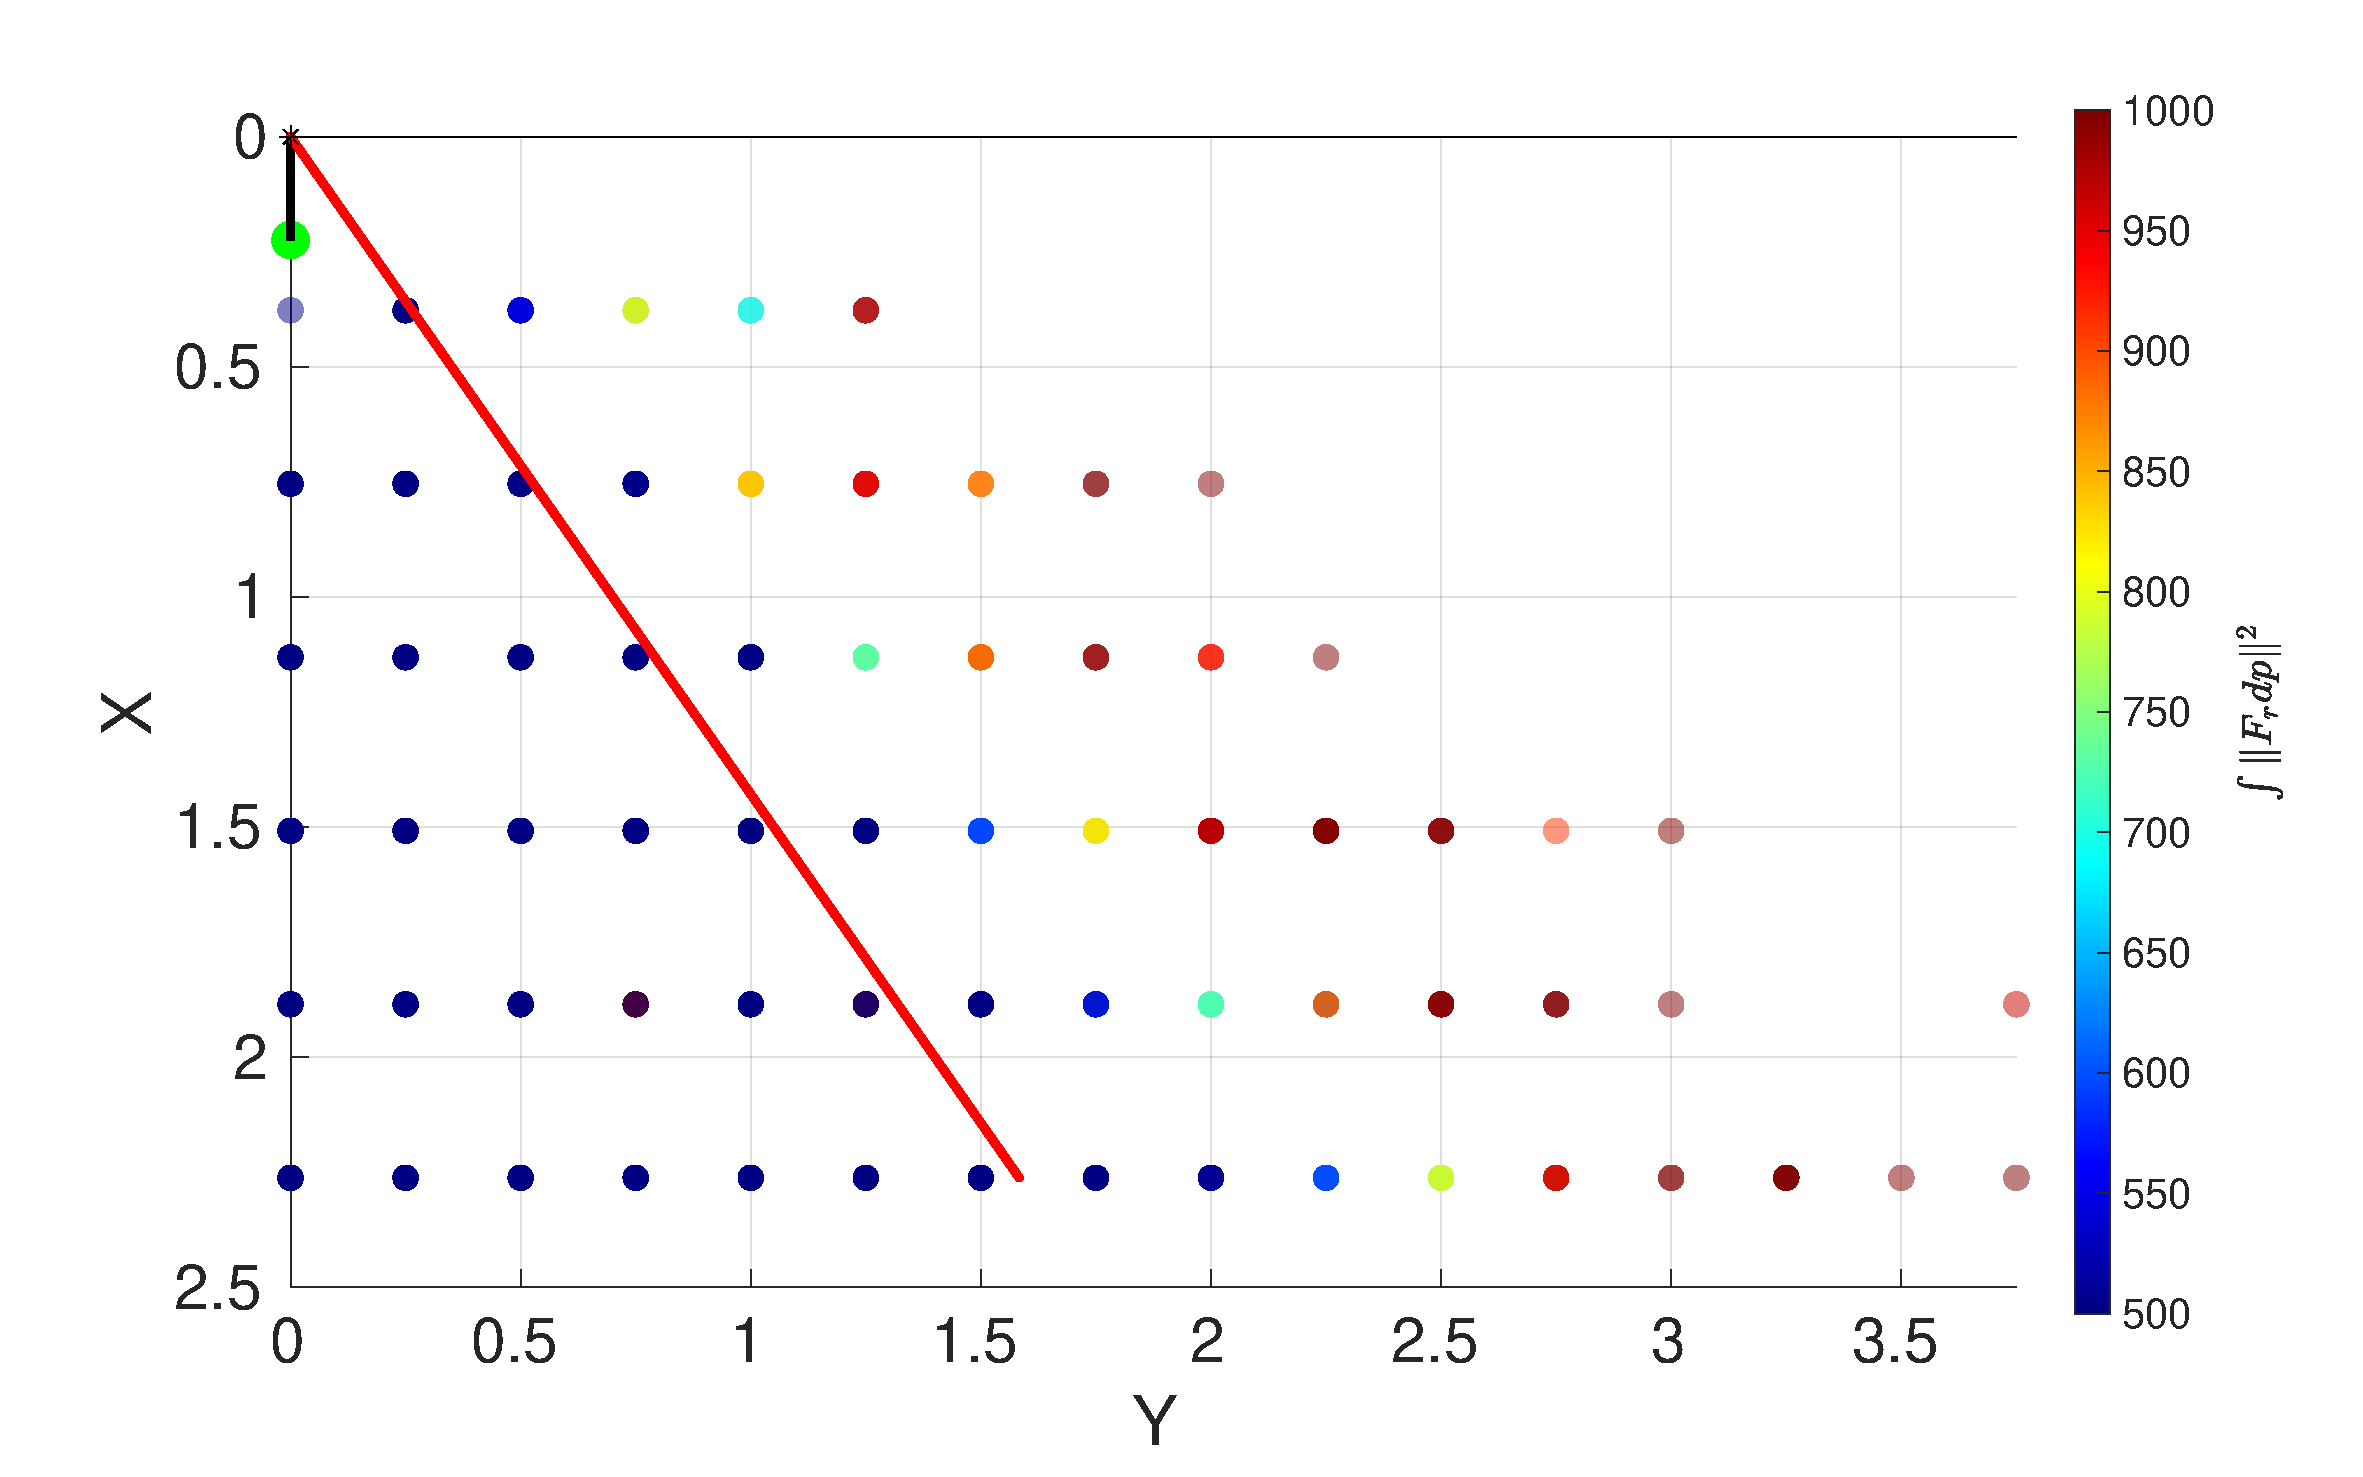
\includegraphics[width=\columnwidth]{matlab/reachable.pdf}
	\caption{\small Simulation. Top view (X-Y plane) of the region of reachable targets for a friction coefficient $\mu =0.7$.
		The black star is the anchor point, the big green dot is the common lift-off point $\vect{p}_0$. The color bar indicates the energy consumed by the winding mechanism to reach the target.}
	\label{fig:reachable_region}
			\vspace{-0.5cm}
\end{figure}
